\documentclass[11pt,a4paper]{article}
\usepackage[T1]{fontenc}
\usepackage[utf8]{inputenc}
\usepackage{lmodern}
\usepackage[margin=2.3cm]{geometry}
\usepackage{graphicx}
\usepackage{booktabs}
\usepackage{longtable}
\usepackage{array}
\usepackage{xcolor}
\usepackage{hyperref}
\usepackage{caption}
\usepackage{float}
\usepackage{enumitem}
\usepackage{fancyvrb}

\hypersetup{colorlinks=true,linkcolor=blue!50!black,urlcolor=blue!50!black}
\setlist{itemsep=1pt,topsep=2pt}
\captionsetup{font=small,labelfont=bf}
\newcommand{\code}[1]{\texttt{\small #1}}
\newcolumntype{L}[1]{>{\raggedright\arraybackslash}p{#1}}
\newcolumntype{R}[1]{>{\raggedleft\arraybackslash}p{#1}}
\graphicspath{{../../docs/figures/}{../screenshots/}}

% Screenshot slot: shows the image when it exists in workshop_2/screenshots/, a framed note otherwise.
\newcommand{\evidence}[2]{%
  \IfFileExists{../screenshots/#1}{%
    \begin{figure}[H]\centering\includegraphics[width=0.9\textwidth]{#1}\caption{#2}\end{figure}}{%
    \begin{center}\fbox{\parbox{0.85\textwidth}{\small\textbf{Screenshot pending:} \texttt{\detokenize{#1}}\\ #2}}\end{center}}}

\title{\textbf{Wildfire Monitoring}\\[2pt]
\large Technical architecture and Bronze/Silver pipeline\\[10pt]
\normalsize Workshop No.~2}
\author{César Ospina (20222020059) \and Santiago Alfonso (20222020093) \and Adrián Espinosa (20222020104)\\
\normalsize Team 3, Computer Engineering, Universidad Distrital Francisco José de Caldas\\
\normalsize Data Analysis Programming, semester 2026-II}
\date{}

\begin{document}
\maketitle

\begin{abstract}
\noindent
This workshop turns the Workshop~1 data contract into a running system. Two Apache Airflow DAGs,
written with the TaskFlow API and running in Docker Compose, move data through two layers.
\code{bronze\_ingestion} polls NASA FIRMS (VIIRS NOAA-20 and NOAA-21, near real time) and the
Open-Meteo forecast every three hours and stores each response untouched inside a JSON envelope in
\code{datalake\_bronze/}. \code{silver\_processing} uses a FileSensor on that folder, applies a
preprocessing pipeline built on the data problems we measured in Workshop~1, and writes typed Parquet
files to \code{datalake\_silver/}, one per topic and run, each row traceable to its Bronze file.
Invalid rows go to a quarantine with a reason, and a state registry makes every run idempotent.
Replaying the recorded Workshop~1 responses through the same code reproduces the Workshop~1 figures
exactly: 1\,109 Colombian detections out of 2\,220, and the same top ten departments.

\medskip\noindent\textbf{Repository:} \url{https://github.com/adriangeb28/wildfire-monitoring}
\end{abstract}

\tableofcontents

\section{Executive summary}

\begin{itemize}
  \item \textbf{Stack.} Docker Compose with Airflow~2.10.5 (webserver, scheduler, triggerer,
        PostgreSQL~16 metadata database) and a PostGIS warehouse that already holds the canonical
        schema from Workshop~1. Six services, one command to start them.
  \item \textbf{Bronze.} Every three hours, three files: one per VIIRS satellite and one for the
        weather of the 33 regions, named \code{<source>\_YYYYMMDD\_HHMMSS.json}. The payload is the
        response as received; the envelope adds its SHA-256, the masked request, the HTTP headers and
        a basic schema check.
  \item \textbf{Silver.} Typed, UTC, validated, region-assigned, deduplicated Parquet:
        \code{fire\_detections\_YYYYMMDD\_HHMMSS.parquet} and
        \code{weather\_hourly\_YYYYMMDD\_HHMMSS.parquet}, plus a quarantine file of rejected rows.
  \item \textbf{Choices.} pandas for Silver (batches of a few thousand rows, rich time-series and
        categorical support); Parquet for persistence (columnar, typed, compressed, read natively by
        PySpark in Workshop~3); a small SQLite registry for idempotency and new/revised detection.
  \item \textbf{Quality.} 19 automated tests run on the recorded Workshop~1 responses, with no
        live calls.
\end{itemize}

\section{Adapting the brief to this hazard}

The workshop brief is written for a pipeline that combines one REST API and one web-scraping target
and that preprocesses free text. Our sources, assigned in the Team Project document, are different:
two REST APIs (FIRMS, CSV; Open-Meteo, JSON) and two archives. We kept every requirement of the brief
and adapted three of them, each for a reason we can show in the data:

\begin{itemize}
  \item \textbf{Web scraping.} None of the four validated sources is a web page; scraping one would
        add a fifth, untested source against the Workshop~1 rule of only adopting sources whose
        access was demonstrated. The Bronze DAG has one extraction task per API source instead.
  \item \textbf{Raw JSON in Bronze.} FIRMS answers in CSV. Converting it to JSON in Bronze would mean
        Bronze is no longer raw. The JSON envelope stores the CSV text unmodified as its
        \code{payload}, so the file is JSON and the data is exactly as received.
  \item \textbf{Text preprocessing for NLP.} The sources contain no free text, only coded fields
        (\code{confidence} = \code{l/n/h}, \code{satellite} = \code{N20/N21}, \code{daynight} =
        \code{D/N}, \code{version} = \code{2.0NRT}). The text step therefore normalises codes
        (trimming, case folding, mapping to controlled vocabularies). Stop words, tokenisation and
        stemming have nothing to act on.
\end{itemize}

\section{Architecture}

\begin{figure}[H]
\centering
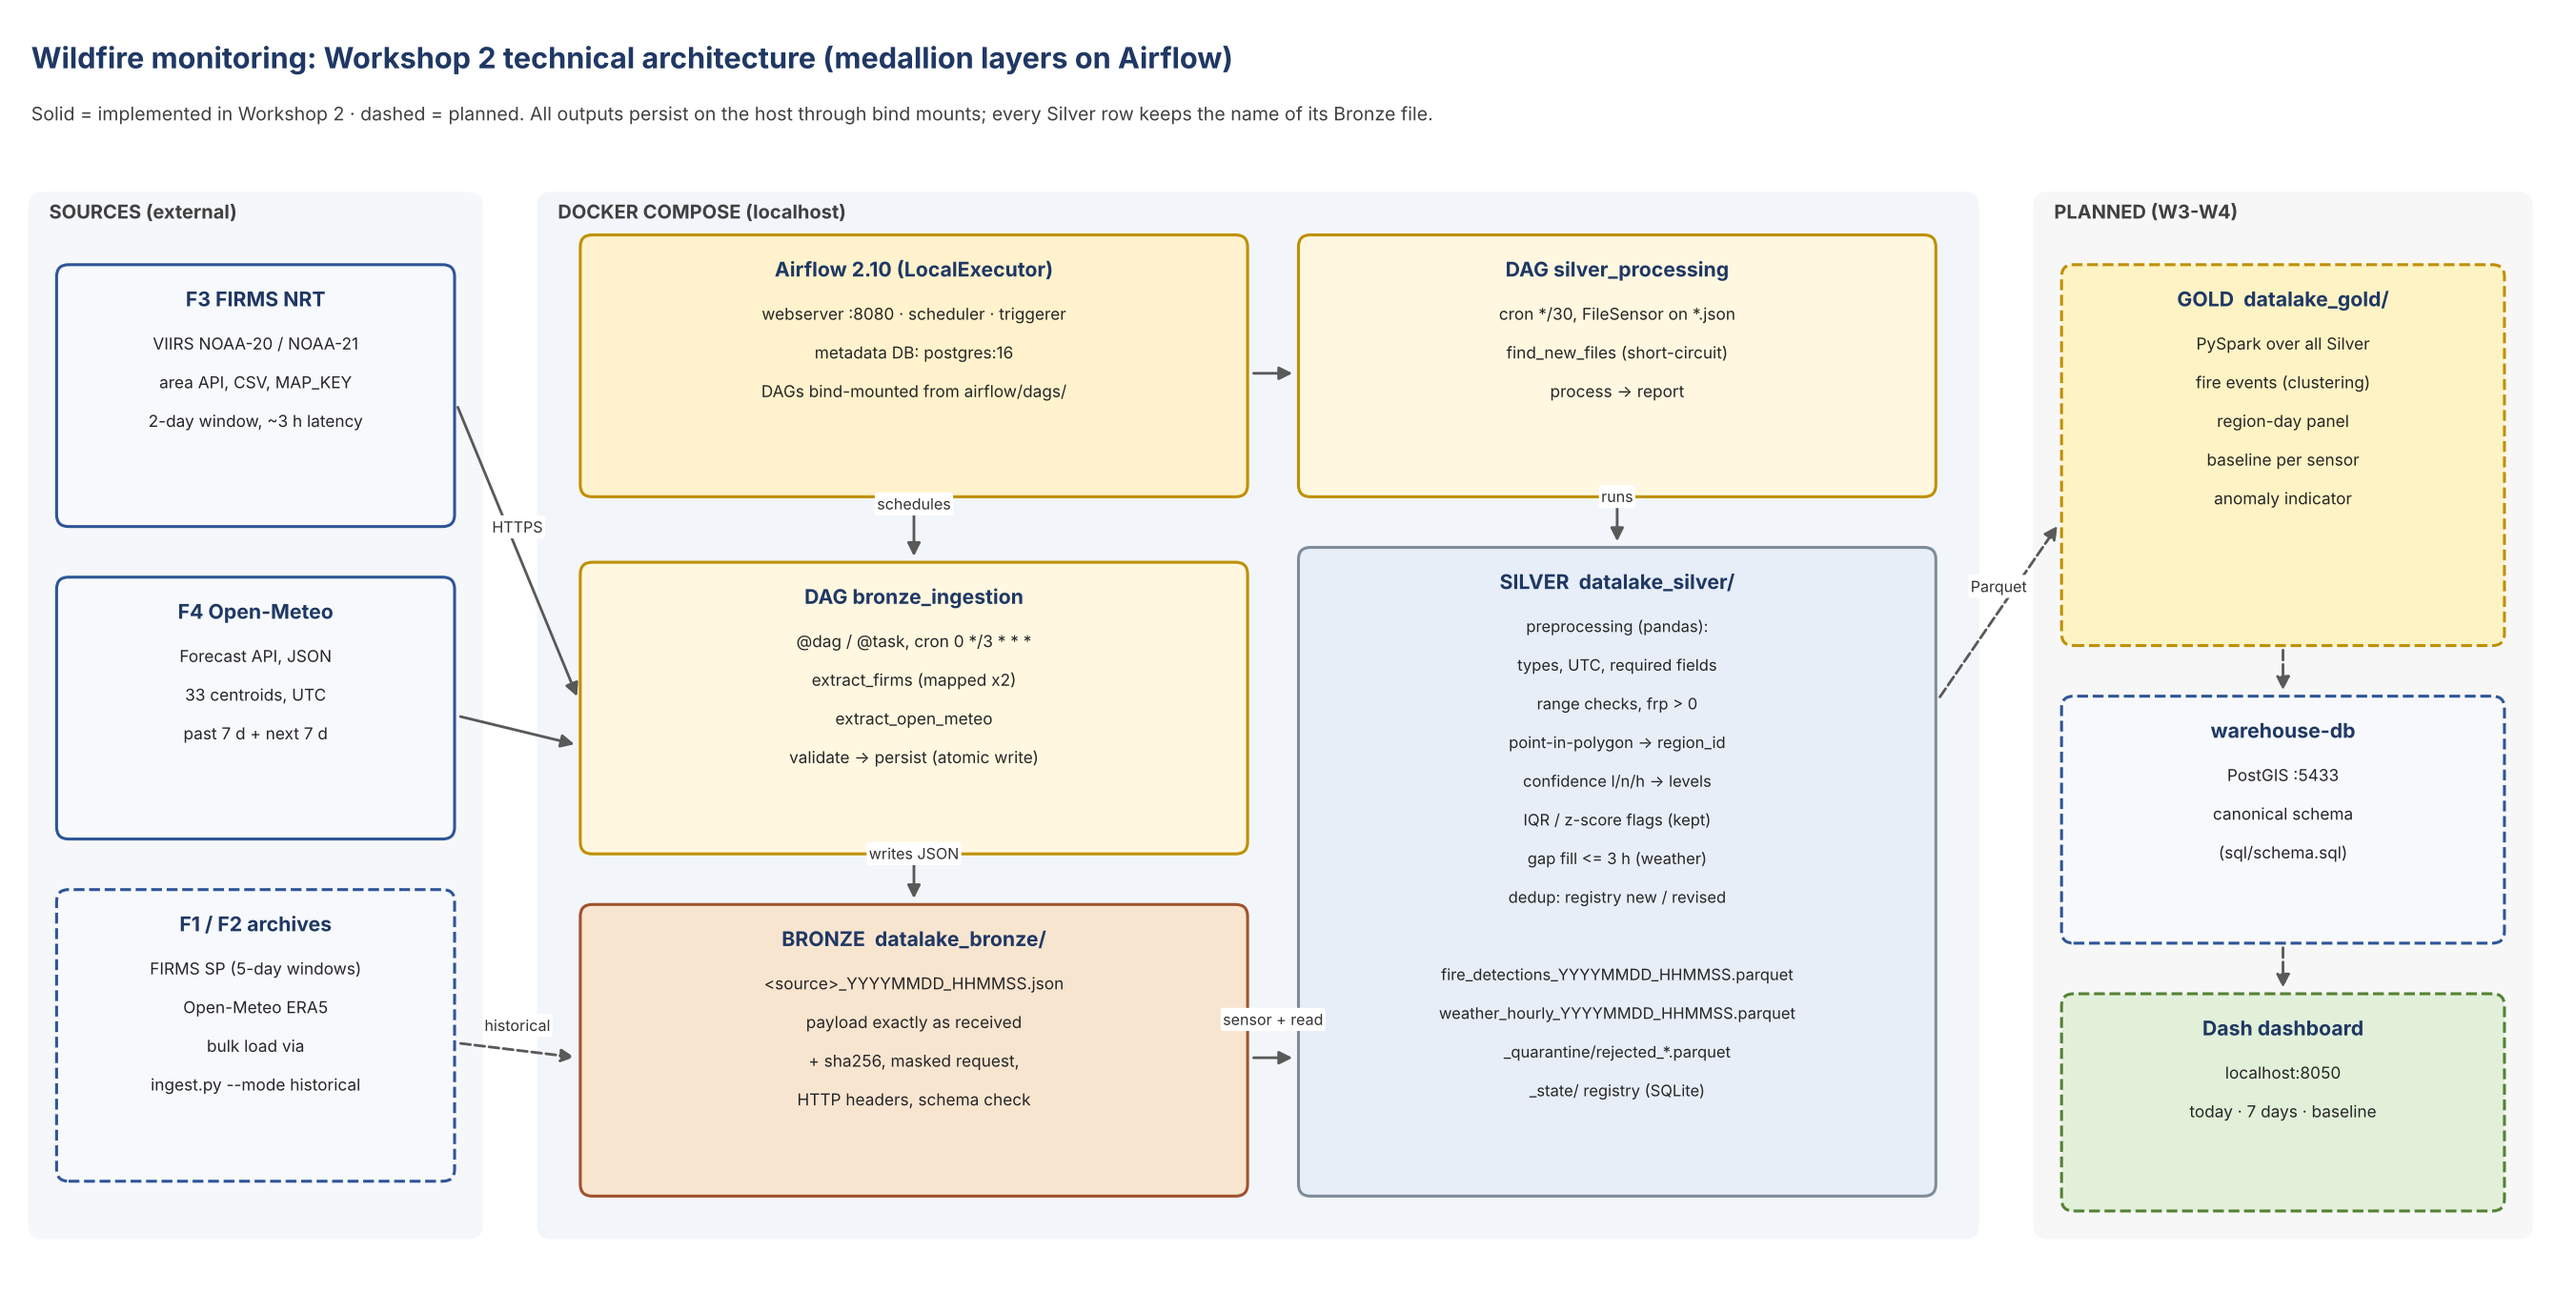
\includegraphics[width=\textwidth]{w2_architecture.png}
\caption{Technical architecture. Solid boxes run in Workshop~2; dashed boxes are planned for
Workshops~3 and~4. Layer boundaries: sources (external), Docker Compose (local), planned.}
\label{fig:arch}
\end{figure}

\begin{longtable}{L{2.8cm}L{3.2cm}L{4.2cm}L{4.4cm}}
\toprule
\textbf{Component} & \textbf{Technology} & \textbf{Input $\rightarrow$ output} & \textbf{Purpose and interactions} \\
\midrule
\endhead
F3 FIRMS NRT & REST, CSV, \code{MAP\_KEY} & bbox + 2-day window $\rightarrow$ CSV & Fire detections about 3~h after the overpass; called by \code{extract\_firms} \\
F4 Open-Meteo & REST, JSON & 33 centroids $\rightarrow$ hourly JSON & Weather context; called by \code{extract\_open\_meteo} \\
Airflow scheduler & Airflow 2.10.5, LocalExecutor & DAG files $\rightarrow$ task runs & Triggers both DAGs on their cron, runs tasks as subprocesses \\
Airflow webserver & Flask UI, :8080 & metadata DB $\rightarrow$ UI & Monitoring, manual triggers, logs \\
Airflow triggerer & Airflow & deferred tasks & Required service; ready for deferrable sensors \\
Metadata DB & PostgreSQL 16 & Airflow state & DAG runs, task instances, XCom \\
\code{bronze\_ingestion} & TaskFlow DAG & APIs $\rightarrow$ Bronze JSON & Extract, validate, persist; every 3~h \\
Bronze layer & JSON files on a bind mount & envelopes & Raw, immutable, replayable provenance \\
\code{silver\_processing} & TaskFlow + FileSensor & Bronze $\rightarrow$ Parquet & Detects files, preprocesses, persists; every 30~min \\
Silver layer & Parquet (PyArrow, snappy) & typed tables & Clean data for Gold; quarantine; registry \\
Gold layer (planned) & PySpark & Silver $\rightarrow$ aggregates & Fire events, region-day panel, indicator \\
\code{warehouse-db} & PostGIS 16-3.4 & \code{sql/schema.sql} & Canonical model, used from Workshop~3 \\
Dashboard (planned) & Plotly Dash :8050 & Gold / DB & Functional user's view \\
\bottomrule
\caption{Components, technologies and interactions.}
\end{longtable}

\paragraph{Technology choices.}
\begin{itemize}
  \item \textbf{pandas over Polars for Silver.} A Bronze batch is at most a few thousand
        detections (2\,220 rows for five days in Workshop~1), far below where Polars' speed matters.
        What matters here is time-zone-aware timestamps, ordered categoricals and per-series
        interpolation, which pandas does directly, and which the rest of the project (Workshop~1
        notebook, indicator validation) already uses.
  \item \textbf{Parquet for Silver.} It is columnar and typed, so the UTC timestamp, the ordered
        confidence category and the boolean flags survive the round trip, which CSV would lose. It is
        compressed (snappy), stores our lineage in its schema metadata, and is what PySpark reads
        natively when Workshop~3 loads all Silver files at once.
  \item \textbf{A JSON envelope for Bronze.} It meets the raw-JSON convention, keeps the original
        bytes, and carries what the incremental design needs: SHA-256 for change detection (FIRMS
        sends no \code{ETag} or \code{Last-Modified}; Workshop~1, Appendix~A), and the fetch time.
  \item \textbf{SQLite registry for Silver state.} Idempotency needs memory across runs (which
        files were processed, which record keys were already written and with what content). One
        file, transactional, in the standard library, and kept on the Silver volume.
  \item \textbf{LocalExecutor.} Two DAGs with a handful of tasks do not need Celery, Redis and
        workers; tasks run as subprocesses of the scheduler. Moving to CeleryExecutor only changes
        the compose file.
\end{itemize}

\paragraph{File nomenclature.}
\begin{itemize}
  \item Bronze: \code{<source>\_YYYYMMDD\_HHMMSS.json}. Sources: \code{firms\_viirs\_noaa20\_nrt},
        \code{firms\_viirs\_noaa21\_nrt}, \code{open\_meteo\_forecast}, and
        \code{firms\_viirs\_noaa20\_sp} for the historical load. The timestamp is the Airflow
        \code{logical\_date} in UTC, so clearing and re-running a run rewrites its own file.
  \item Silver: \code{<topic>\_YYYYMMDD\_HHMMSS.parquet} with the processing-run time in UTC. Topics:
        \code{fire\_detections}, \code{weather\_hourly}.
  \item Quarantine: \code{\_quarantine/rejected\_YYYYMMDD\_HHMMSS.parquet}.
\end{itemize}

\section{Preprocessing pipeline}

Every rule answers a problem we measured in Workshop~1 (report, Table~3, and
\code{workshop\_1/findings.md}). The code is \code{src/pipeline/preprocess.py}; its docstrings
repeat this table so the rules and the code cannot drift apart.

\subsection{Fire detections (F3)}

\begin{longtable}{L{2.6cm}L{5.6cm}L{6.3cm}}
\toprule
\textbf{Step} & \textbf{Rule} & \textbf{Evidence from Workshop 1} \\
\midrule
\endhead
Code normalisation & Trim and case-fold \code{confidence}, \code{satellite}, \code{daynight}, \code{instrument} & Coded fields only; no free text to tokenise \\
Types & Numeric fields to float; \code{acq\_time} zero-padded to HHMM, then \code{observed\_at} = \code{acq\_date} + time, UTC & 436 night rows had a 3-digit \code{acq\_time} (658 = 06:58); read as an integer it becomes minutes or hours \\
Required fields & Missing latitude, longitude, \code{acq\_date}, \code{acq\_time}, satellite or FRP $\rightarrow$ quarantine (\code{missing\_*}, \code{bad\_acq\_time}); never imputed & Imputing a position or time would invent a detection \\
Validation & Coordinates in range and inside the bbox; FRP $>$ 0; clock time valid; not in the future & 1 row with FRP = 0.00 \\
Region & Point-in-polygon on the 33 regions; outside $\rightarrow$ quarantine \code{outside\_colombia} & Only 50.0\,\% of the 5-day bbox rows and 33.7\,\% of 2024 are Colombian \\
Optional fields & \code{bright\_ti4/ti5} outside 200--400~K $\rightarrow$ null + flag; null scan, track, brightness stay null; null confidence $\rightarrow$ \code{unknown} & They do not enter the indicator; no reason to invent them \\
Confidence & \code{l/n/h} $\rightarrow$ ordered category \code{low $<$ nominal $<$ high}; raw code kept & \code{confidence $>$ 50} kept 0 of 2\,220 VIIRS rows \\
Outliers & Flag, never delete: IQR fence on $\log_{10}$ FRP per satellite (primary, $Q_3 + 1.5\,IQR$, $n \ge 20$) and z-score on $\log_{10}$ FRP (stored) & FRP median 4.8~MW, max 196~MW; the 196~MW fire is real (seen three times) \\
Duplicates & In batch: exact key (source, satellite, lat, lon, \code{observed\_at}) $\rightarrow$ keep first. Across batches: registry by \code{event\_id} and \code{content\_hash} $\rightarrow$ duplicate dropped, changed values kept as \code{revised} & The 1-day polling overlap returns the same rows twice; NRT values can be revised \\
Near-duplicates & Kept: several detections of one fire, grouped in Gold & 44.5\,\% share a $\sim$1~km cell; they are not copies \\
Schema & 28 typed columns, 10 required; any null in a required column fails the run & Table~\ref{tab:schema} \\
\bottomrule
\caption{Fire-detection preprocessing.}
\end{longtable}

\subsection{Weather (F4)}

\begin{longtable}{L{2.6cm}L{6.2cm}L{5.7cm}}
\toprule
\textbf{Step} & \textbf{Rule} & \textbf{Reason} \\
\midrule
\endhead
Shape & Long format: one row per region, hour and variable & A weather value is a series sample, not an event (W1, problem 8) \\
Time & Request forced to \code{timezone=UTC}; parsed as UTC & Without it the API returns local time, a silent 5-hour shift (W1, problem 7) \\
Ranges & Temperature $-30$--50~°C, humidity 0--100\,\%, precipitation 0--200~mm/h, wind 0--250~km/h; outside $\rightarrow$ null + \code{out\_of\_range} & Physical sanity, not climatology \\
Nulls & Gaps $\le$ 3 consecutive hours: linear interpolation, \code{imputed = true}; longer gaps stay null (\code{missing}) & A short gap in a smooth series is safely bridged; a long one would be invented \\
Outliers & $|z| > 4$ inside each region-variable series $\rightarrow$ flag only; not applied to precipitation & Precipitation is zero-inflated; a z-score would flag every shower \\
Duplicates & Key (region, hour, variable); the registry keeps changed forecasts as \code{revised} & Each poll repeats 13 of its 14 days, and forecasts change \\
\bottomrule
\caption{Weather preprocessing.}
\end{longtable}

\subsection{Silver schema}

\begin{table}[H]
\centering
\small
\begin{tabular}{L{3.0cm}L{3.0cm}L{8.5cm}}
\toprule
\textbf{Column} & \textbf{Type} & \textbf{Meaning} \\
\midrule
\code{event\_id} & string, required & SHA-256 (32 hex) of source, satellite, lat, lon (5 dp), \code{observed\_at} \\
\code{observed\_at} & timestamp UTC, required & Detection time \\
\code{latitude}, \code{longitude} & float64, required & WGS84 decimal degrees \\
\code{region\_id}, \code{region\_name} & string, required / optional & ISO 3166-2 code (\code{CO-NSA}) and name \\
\code{frp} & float64, required & Fire Radiative Power, MW (unit in the file metadata) \\
\code{bright\_ti4}, \code{bright\_ti5} & float64 & Brightness temperature, K \\
\code{satellite}, \code{instrument}, \code{daynight} & category & Codes \\
\code{confidence\_raw}, \code{confidence\_level} & string, ordered category & As received, and normalised \\
\code{frp\_outlier}, \code{frp\_log\_z}, \code{quality\_flags} & bool, float64, string & Outlier flag, z-score, semicolon-separated flags \\
\code{content\_hash}, \code{record\_status} & string & Change detection; \code{new} or \code{revised} \\
\code{bronze\_file}, \code{bronze\_row} & string, int64 & Lineage: Bronze file and CSV line \\
\code{processed\_at} & timestamp UTC & Silver run time \\
\bottomrule
\end{tabular}
\caption{\code{fire\_detections} schema (main columns; 28 in total). \code{weather\_hourly} has 15:
key, region, hour, variable, value, unit, forecast flag, lead time, imputed flag, quality flags, hash,
status and lineage.}
\label{tab:schema}
\end{table}

\section{Docker stack}

\begin{table}[H]
\centering
\small
\begin{tabular}{L{3.2cm}L{4.0cm}L{7.3cm}}
\toprule
\textbf{Service} & \textbf{Image} & \textbf{Role} \\
\midrule
\code{postgres} & \code{postgres:16} & Airflow metadata database (named volume \code{airflow-db}) \\
\code{airflow-init} & project image & One-shot: folders and permissions, \code{airflow db migrate}, admin user \\
\code{airflow-webserver} & project image & UI and API on \code{localhost:8080} \\
\code{airflow-scheduler} & project image & Schedules and executes tasks (LocalExecutor) \\
\code{airflow-triggerer} & project image & Deferrable operators \\
\code{warehouse-db} & \code{postgis/postgis:16-3.4} & Canonical schema loaded at first start, \code{localhost:5433} \\
\bottomrule
\end{tabular}
\caption{Services in \code{docker-compose.yml}. The project image is \code{apache/airflow:2.10.5-python3.11}
plus pandas, PyArrow, Shapely, requests, python-dotenv and PyYAML, installed against Airflow's
official constraints file.}
\end{table}

\paragraph{Volumes.} Bind mounts: \code{airflow/dags} (live DAG reload), \code{airflow/logs},
\code{airflow/plugins}, \code{src} (the pipeline package, on \code{PYTHONPATH}), \code{config},
\code{reference} (region layer), and \code{datalake\_bronze}, \code{datalake\_silver},
\code{datalake\_gold}, so every output stays on the host when the containers stop. Named volumes hold
the two databases.

\paragraph{Networking.} All services share the default Compose network and reach each other by service
name (\code{postgres}). Only two ports are published: 8080 (Airflow UI) and 5433 (warehouse). The
FileSensor's base path is an Airflow connection defined as an environment variable
(\code{AIRFLOW\_CONN\_FS\_BRONZE}), so no manual setup is needed in the UI.

\paragraph{Secrets.} \code{FIRMS\_MAP\_KEY} comes from \code{.env} through \code{env\_file}; the
file is git-ignored and the Bronze envelope stores the request URL with the key masked.

\paragraph{Setup.}
\begin{Verbatim}[fontsize=\small]
cp .env.example .env            # set FIRMS_MAP_KEY
docker compose build
docker compose up airflow-init
docker compose up -d            # http://localhost:8080  (airflow / airflow)
\end{Verbatim}

\section{DAGs}

\subsection{\code{bronze\_ingestion}}

\begin{itemize}
  \item \textbf{Schedule:} \code{0 */3 * * *}, the three-hour polling frequency of the Workshop~1
        contract (FIRMS NRT latency). \code{catchup=False}, one active run at a time, two retries with
        exponential back-off, plus a second back-off layer inside the HTTP client (5, 10, 20~s on
        network errors and 429/5xx).
  \item \textbf{Tasks:} \code{extract\_firms} is mapped over the two VIIRS products (dynamic task
        mapping) and asks for the 2-day window ending at the run (1-day overlap);
        \code{extract\_open\_meteo} makes one call for the 33 centroids. Each feeds \code{validate}
        (header and required columns for CSV; block count, time zone and variables for JSON) and
        \code{persist} (atomic write).
  \item \textbf{Errors:} a failed schema check is still persisted, with \code{ok = false}, so the
        evidence is kept, and then the task fails so the run is visibly red. An empty window is valid
        (no overpass yet) and is recorded as \code{empty\_window}.
  \item \textbf{Output:} three JSON files per run.
\end{itemize}

\subsection{\code{silver\_processing}}

\begin{itemize}
  \item \textbf{Trigger:} scheduled every 30 minutes; the first task is a \code{FileSensor} on
        \code{datalake\_bronze/*.json}. The sensor uses \code{mode="reschedule"} (no worker slot held
        while waiting), \code{poke\_interval=120}~s, and \code{timeout=3}~h, one Bronze period, after
        which it soft-fails (skipped, not failed).
  \item \textbf{Newness:} a FileSensor answers whether a file exists, not whether it is new. The
        short-circuit task \code{find\_new\_files} compares the folder with the registry (file name
        and SHA-256); when nothing is new, the rest of the run is skipped and nothing is written.
  \item \textbf{Processing:} \code{process} runs the preprocessing, classifies records against the
        registry, writes the Parquet files and commits the registry in one transaction;
        \code{report} logs the outputs and totals.
  \item \textbf{Failure safety:} Parquet is written before the registry commit; at the next start,
        any Parquet file the registry does not know (a run that died in between) is deleted, so a
        crash cannot leave duplicated rows.
  \item \textbf{Lineage:} every row has \code{bronze\_file} and \code{bronze\_row}; the Parquet
        schema metadata lists the run's Bronze files, the pipeline version and the units;
        \code{datalake\_silver/\_manifest.jsonl} keeps one line per run.
\end{itemize}

\section{Results}

\subsection{Offline end-to-end run on the recorded responses}

Before running against the live APIs, we replayed the three responses recorded in Workshop~1
(\code{python ingest.py --mode incremental --from-fixtures}) through the same Silver code:

\begin{table}[H]
\centering
\small
\begin{tabular}{L{6.2cm}R{2.4cm}L{5.6cm}}
\toprule
\textbf{Measure} & \textbf{Value} & \textbf{Check} \\
\midrule
FIRMS rows in (NOAA-20 + NOAA-21, 5 days) & 2\,220 & = Workshop~1 \\
Rows in \code{fire\_detections} (Colombia) & 1\,109 & = Workshop~1 (50.0\,\%) \\
Quarantined \code{outside\_colombia} & 1\,110 & \\
Quarantined \code{frp\_nonpositive} & 1 & = Workshop~1 problem 3 \\
FRP outliers flagged and kept & 14 & incl. the 196~MW fire \\
Rows in \code{weather\_hourly} (Bogotá, 96~h $\times$ 4 variables) & 384 & 0 nulls, 0 imputed \\
Second run on the same files & nothing written & idempotent \\
\bottomrule
\end{tabular}
\caption{Offline replay. The top ten departments match the Workshop~1 notebook exactly
(Norte de Santander 175, Antioquia 143, Vichada 133, \ldots).}
\end{table}

\subsection{Tests}

\code{tests/test\_pipeline.py} has 19 tests on the recorded responses: Bronze schema check, empty
window, tamper detection by SHA-256, \code{acq\_time} padding, every quarantine reason, confidence
levels, brightness sanity, in-batch duplicates, the 196~MW fire kept and flagged, weather gap filling,
schema enforcement, Silver idempotency, cross-batch duplicate and revision detection, orphan cleanup,
lineage, and a real Parquet round trip.

\subsection{Live runs in Airflow (2026-11-17, UTC)}

The stack was built and started with Docker Desktop on Windows. \code{bronze\_ingestion} ran three
times (the scheduled 21:00 run and two manual triggers at 02:46~UTC), producing nine Bronze files
(three per source, 58--70~KB per FIRMS file, 431~KB per forecast file). \code{silver\_processing}
processed the first round at 02:45~UTC:

\begin{table}[H]
\centering
\small
\begin{tabular}{L{6.8cm}R{2.4cm}}
\toprule
\textbf{Measure (live run)} & \textbf{Value} \\
\midrule
FIRMS rows in (NOAA-20 827, NOAA-21 675) & 1\,502 \\
Rows in \code{fire\_detections\_20261117\_024528.parquet} & 687 \\
Quarantined \code{outside\_colombia} & 815 \\
Rows in \code{weather\_hourly\_20261117\_024528.parquet} (33 regions $\times$ 336~h $\times$ 4) & 44\,352 \\
\bottomrule
\end{tabular}
\caption{First live Silver run (02:45~UTC). A second Silver run at 02:54~UTC processed the six Bronze
files of rounds two and three: every fire and weather row in them had already been written (same
FIRMS window and same forecast hour, polled minutes apart), so the registry classified all of them as
duplicates and the run wrote schema-valid files with 0 new rows, plus 1\,630 quarantined rows. This is
the cross-batch deduplication working as designed; new rows only appear when polls are hours apart.}
\end{table}

All outputs are committed in \code{datalake\_bronze/}, \code{datalake\_silver/} and
\code{datalake\_silver/\_quarantine/}.

\evidence{02_airflow_dags.png}{Airflow UI with both DAGs.}
\evidence{03_bronze_graph.png}{Successful \code{bronze\_ingestion} run (graph view).}
\evidence{05_silver_graph.png}{Successful \code{silver\_processing} run (02:54~UTC): FileSensor, short-circuit, processing of the six pending Bronze files of rounds two and three, and report.}
\evidence{07_silver_idempotent.png}{A second Silver run on the same files: skipped by the short-circuit.}
\evidence{08_bronze_runs.png}{Three or more Bronze runs (grid view).}
\evidence{09_folders.png}{Nine Bronze JSON files from three runs on the host.}
\evidence{09b_folders.png}{Silver Parquet files, manifest, quarantine and state folders on the host.}

\section{Challenges and decisions}

\begin{itemize}
  \item \textbf{A brief written for other sources.} Web scraping and NLP do not apply; we adapted
        them openly (Section~2) instead of adding an untested source to tick a box.
  \item \textbf{CSV in a JSON layer.} Solved with the envelope: raw bytes, JSON container.
  \item \textbf{A FileSensor does not know what is new.} It only sees that files exist. We kept the
        sensor as the arrival gate and added a registry check as the newness gate; a custom sensor
        on the registry is the planned refinement.
  \item \textbf{Idempotent file names.} Wall-clock names would create a new Bronze file on every
        retry. Bronze uses the run's \code{logical\_date}; Silver uses the processing time, as the
        brief requires, and relies on the registry for idempotency.
  \item \textbf{Overlap and revisions.} The 1-day overlap is the recovery policy of Workshop~1, so
        duplicates across batches are expected. The registry distinguishes a repeat (dropped) from a
        revision (kept, \code{revised}), which is the new/changed detection the course asks for.
  \item \textbf{No HTTP change metadata.} FIRMS sends no \code{ETag} or \code{Last-Modified}; the
        SHA-256 per payload and the content hash per row replace them.
  \item \textbf{Region layer inside the containers.} The 8.9~MB boundary file was git-ignored. It is
        now versioned in \code{reference/} with coordinates rounded to 4 decimals ($\sim$11~m),
        5.5~MB, so the containers need no download step.
\end{itemize}

\section{Next steps (Workshop 3)}

Gold layer with PySpark over all Silver files: fire events by spatio-temporal grouping, the
region-day panel, the per-sensor baseline and the weather-conditioned indicator; historical load of
the SP archive and ERA5 into Bronze and Silver; load into the PostGIS warehouse.

\section*{References}
\begin{itemize}
  \item Apache Airflow 2.10 documentation: TaskFlow API, FileSensor, Docker Compose quick start.
        \url{https://airflow.apache.org/docs/apache-airflow/2.10.5/}
  \item NASA FIRMS / LANCE, NASA EOSDIS. Area API. \url{https://firms.modaps.eosdis.nasa.gov/api/area/}
  \item Open-Meteo Forecast API (CC BY 4.0, ``Weather data by Open-Meteo.com'').
        \url{https://open-meteo.com/en/docs}
  \item Apache Parquet and Apache Arrow (PyArrow). \url{https://parquet.apache.org},
        \url{https://arrow.apache.org/docs/python/}
  \item pandas. \url{https://pandas.pydata.org}; Shapely. \url{https://shapely.readthedocs.io}
  \item geoBoundaries, \code{gbOpen/COL/ADM1} (ODbL 1.0). \url{https://www.geoboundaries.org}
  \item Docker Compose. \url{https://docs.docker.com/compose/}
\end{itemize}

\end{document}
